\section{Basic Concepts}
\stlabel{basic}

\GROOVE shows rules and graphs using various kinds of graphical embellishments,
such as colours, bold and italic fonts, dashed and dotted outlines, and special
symbols. During editing, however, the node and edge labels you enter do not
have those embellishments. Instead, you have to use a fairly rich textual
syntax to make the same distinctions. The prime element in this syntax is a
\emph{prefix}, usually consisting of an identifier followed by a colon (`:').

\begin{table}
\begin{minipage}{\textwidth}
\begin{center}
\begin{tabular}{|l|c|l|l|}
\hline\hline
\bf Prefix
 & \bf Where?\footnote{Abbreviations:
on \textsf{N}ode / \textsf{E}dge, resp.\ in \textsf{H}ost
graph / \textsf{R}ule / \textsf{T}ype graph}
 & \bf Explanation
 & \bf Sample\footnote{Name of a sample rule system in which this is used, see
 \url{http://sf.net/projects/groove}, samples download} \\
\hline
\remP & \sf NE,HRT
 & Remark node or edge; used for documentation purposes
 & \textsf{attributed-graphs} \\
\hline
\useP & \sf NE,R
 & Declares a node or edge to be a reader (the default value)
 & \\
\delP & \sf NE,R
 & Declares a node or edge to be an eraser
 & \\
\newP & \sf NE,R
 & Declares a node or edge to be a creator
 & \\
\cnewP & \sf NE,R
 & Declares a node or edge to be a conditional creator
 & \\
\notP & \sf NE,R
 & Declares a node or edge to be an embargo
 & \\
\hline
\boolP & \sf NE,HRT
 & On nodes, a boolean value or type; on edges, a boolean operator
 & \\
\intP & \sf NE,HRT
 & On nodes, an integer value or type; on edges, an integer operator
 & \\
\realP & \sf NE,HRT
 & On nodes, a real value or type; on edges, a real operator
 & \\
\stringP & \sf NE,HRT
 & On nodes, a string value or type; on edges, a string operator
 & \\
\argP & \sf E,R
 & Argument edge, from a product node to an attribute value
 & \textsf{attributed-graphs} \\
\prodP & \sf N,R
 & Product node, collecting arguments for an attribute operation
 & \textsf{attributed-graphs} \\
\letP & \sf N,HR
 & Syntactic sugar for attribute assignment
 & \textsf{attributed-graphs} \\
\testP & \sf N,R
 & Attribute condition that must be satisfied for a rule to apply
 & \textsf{attributed-graphs} \\
\hline
\parP & \sf N,R
 & Anonymous or numbered rule parameter node
 & \textsf{parameters} \\
\parinP & \sf N,R
 & Numbered rule input parameter node
 & \\
\paroutP & \sf N,R
 & Numbered rule output parameter node
 & \\
\hline
\absP & \sf NE,T
 & Abstract type node or edge
 & \\
\subP & \sf E,T
 & Inheritance edge between node types
 & \textsf{inheritance} \\
\inP & \sf E,T &
Incoming edge multiplicity declaration
 & \\
\outP & \sf E,T &
Outgoing edge multiplicity declaration
 & \\
\partP & \sf E,T &
Composite edge declaration
 & \\
\importP & \sf N,T &
Indicates that the node is imported from another type graph
 & \\
\hline
\forallP & \sf N,R
 & Universal quantifier node
 & \\
\forallxP & \sf N,R
 & Non-vacuous universal quantifier node
 & \\
\existsP & \sf N,R
 & Existential quantifier node
 & \\
\existsxP & \sf N,R
 & Optional existential quantifier node
 & \\
\nestedP & \sf E,R
 & Quantifier nesting edge
 & \\
\hline
\idP & \sf N,R &
User-defined node identity
 & \\
\hline
\colorP
 & \sf N,RT
 & Defines the text and outline colour of a node or node type
 & \textsf{colours} \\
\edgeP & \sf N,T
 & Defines a node type to be a nodified edge
 & \textsf{bridge} \\
\hline
\pathP & \sf E,R &
Declares the remainder of the text to be a regular expression label
 & \\
\litP & \sf NE,HR &
Declares the remainder of the text to be a literal edge label
 & \\
\typeP & \sf NE,HRT &
Declares the remainder of the text to be a node type
 & \\
\flagP & \sf NE,HRT &
Declares the remainder of the text to be a flag (= node label)
 & \\
\hline\hline
\end{tabular}
\end{center}
\end{minipage}
\caption{Overview of available edit prefixes. (See also the syntax help in the
\GROOVE Simulator).}
\end{table}


%%% Local Variables: 
%%% mode: latex
%%% TeX-master: "usermanual"
%%% End: 


\subsection{Graphs}
\stlabel{Graphs}

\GROOVE is based on directed node- and edge-labelled graphs. Graph nodes are
depicted as boxes, and edges as arrows between them; the node labels are
inscribed in the nodes, the edge labels along or on top of the arrows.

There are two kinds of node labels: types and flags. In the Edit view, these
are distinguished from one another and from edge labels by prefixing them with
``\typeP'' and ``\flagP'', respectively. If you omit the prefix, \GROOVE will
interpret the label as an edge label, and it will create a self-edge with that
label. (If you have no types or flags in your graph, self-edge labels remain
inscribed in the nodes in the Display view.) In the Display view, types are set
bold and flags are set italic. Here is an example:

\views{basic-graph}

\paragraph{Type and flag labels.}

As seen above, node labels can be either types or flags. There are two
important differences:
\begin{itemize}\noitemsep
\item Type labels are partially ordered by subtyping (often called
  inheritance). This affects rule matching: a type label in a rule matches all
  subtype labels (i.e., those that are smaller in the partial ordering) of the
  host graph.
\item If a type graph is used, type labels must be unique: every node must have
  exactly one type label.
\end{itemize}

\paragraph{Graph label syntax.}

Node labels are restricted to identifiers; i.e., strings of characters starting
with a letter or underscore, and containing only letters, digits, underscores
or dollar signs. It is also recommended, but not enforced, to use only
identifiers as edge labels. If you want to use other labels, start the label
(in the Edit view) with a colon (``\lab{:}''). The colon will not be part of
the actual label: it is an escape character indicating that what follows should
be taken literally. (Thus, an initial colon serves as an ``escape'' character
precisely as an initial single quote serves as an escape in Excel.) Whitespace
other than simple spaces, such as tabs and newlines, cannot be included in
labels.

\subsection{Rules}
\stlabel{rules}

Formally, rules consist of left hand sides, right hand sides and negative
application conditions (NACs), all of which are different graphs, connected by
morphisms. In \GROOVE{} these graphs are combined into one single view, and
colour coding is used to distinguish the original components. As a consequence,
a \GROOVE{} view of a rule has the following kinds of elements:

\begin{description}
\item[Readers.] These are nodes and edges that are in both the LHS and the RHS.
  In both the editor and the display view, they are depicted just like ordinary
  graph elements; hence, the outlines are thin and black and the font colour is
  black. In the Edit view, the fact that an edge is a reader may be indicated
  explicitly by including an (optional) prefix ``\useP'' in front of the label.

\item[Erasers.] These are nodes and edges that occur in the LHS but not the
  RHS, meaning that they must be matched in order for the rule to apply, but by
  applying the rule they will be deleted. In the Display view, such elements
  are depicted by a thin, dashed blue outline and blue text; moreover, erased
  node labels (on non-erased nodes) are prefixed with ``lab{--}''. In the
  Edit view, erasers are distinguished by a special prefix ``\delP''. For
  eraser nodes, this prefix should appear \emph{on its own} as a node label;
  for eraser edges, the prefix is followed by the edge label.

\item[Creators.] These are nodes and edges that occur in the RHS but not the
  LHS, meaning that they will be created when the rule is applied. In the
  Display view, such elements are depicted by a slightly wider, solid green
  outline (light grey in a black-and-white representation) and green text;
  moreover, created node labels (on non-created nodes) are prefixed with
  ``lab{+}''. In the Edit view, creators are distinguished by a special
  prefix ``\newP''. For creator nodes, this prefix should appear \emph{on its
  own} as a node label; for creator edges, the prefix is followed by the edge
  label.

\item[Embargoes.] These are nodes and edges that are in a NAC, but not in the
  LHS. This means that they \emph{forbidden}: their presence in the host graph
  will prevent the rule from being applied. In the Display view, such elements
  are depicted by a wide, dashed red outline (darker grey in a black-and-white
  representation) and red text; moreover, forbidden node labels (on non-embargo
  nodes) are prefixed with ``\lab{!}''. In the Edit view, creators are
  distinguished by a special prefix ``\notP''. For embargo nodes, this prefix
  should appear \emph{on its own} as a node label; for embargo edges, the
  prefix is followed by the edge label.
\end{description}
%
If a node plays any of the roles of eraser, creator or embargo, its incident
edges implicitly also have this role. Thus, in that case the corresponding
prefix can be omitted in the Edit view.

\medskip\noindent The following rule example contains all of the above types of
elements:

\views{simple-rule}

Note that, among other things, this rule specifies the deletion and creation of
a type label; this is something that is forbidden in the presence of a type
graph (see \stref{typing}).

\paragraph{Rule label syntax.}

Label parsing in rules is more complicated than in graphs, because there are
many more special labels (see below for a discussion). The following points
should be noted.
%
\begin{itemize}\noitemsep
\item The rule for the use of colons is the same as for graphs: when an
  (unquoted) colon is used as part of a label, there should be a single initial
  colon preceding the entire label; this initial colon is not considered to be
  part of the label itself.

\item In addition to the above, whenever the spacial characters \lab{'}
  (single quote), \lab{\textbackslash} (backslash), \lab{?} (question
  mark), \lab{!}  (exclamation mark), \lab{=} (equality sign), or
  \lab{\{} and \lab{\}} (opening and closing curly braces) are used
  literally within labels, i.e., not in their role as special characters, the
  whole label must be single-quoted. The surrounding single quotes are
  themselves not considered to be part of the label.

\item The backslash (``\lab{\textbackslash}'') serves as an escape character
  within a single-quoted label: any next character (including the backslash
  itself) is interpreted literally rather than as a special character. This is
  especially needed to use single quotes within single-quoted labels.
\end{itemize}
%
For instance, the label \lab{'\textbackslash\textbackslash?\textbackslash''}
(ending on two single quotes) in a rule matches the label
\lab{\textbackslash?'} in a graph.

\paragraph{Rule names.}

Rules have names. The names are essentially identifiers. The actual constraints
on rule names are quite flexible: any string that can be used as a file name
but does not contain spaces or periods is allowed as a rule name. However, it
is \emph{recommended} to stick to rule names that are valid identifiers:
%
\begin{itemize}\noitemsep
\item Start a rule name with a letter --- by convention a small letter;
\item Restrict the remaining characters to letters, digits, underscores or
  dollar characters.
\end{itemize}
%
Rule names can impose a hierarchical structure, similar to the package
structure of qualified Java class names. For instance, the name
``$\lab{a.b}$'' stands for rule ``\lab{b}'' in package
``\lab{a}''. This mechanism is only there for the purpose of structuring
larger sets of rules; the structure does not change the meaning of the rule
system (see also \stref{trans} below).

\paragraph{Example usage.}

The use of the above features is demonstrated by the following \GROOVE samples:
%
\begin{itemize}\noitemsep
\item \textsf{circular-buffer}, a simple data structure with two rules,
  containing creators, erasers and embargoes;
\item \textsf{loose-nodes}, showing that node labels are just self-edges which
  can be added to existing, non-labelled nodes.
\end{itemize}

\subsection{Negations}
\stlabel{negation}

Another way to forbid an edge, type or flag is by inserting an exclamation mark
in front of its label. This therefore has the same effect as the ``\notP''
prefix, but it can only be used for edges. Moreover, negations can also be used
\emph{within} embargoes, achieving a double negation. For instance, the
following rule can only match if the \tlab{Bus} has not already started
(\rlab{!flag:start}-edge), and there is \emph{no} \tlab{Pupil} that is
\emph{not} in the bus (\rlab{!in}-embargo edge) --- in other words, if all the
pupils are in the bus.

Note that in the display view, all negations are displayed as binary edges
(including the \rlab{!flag:start}-edge), and they are typeset in italic. This
is because they are actually special cases of regular expression edges; see
\stref{regular} below.

\views{double-negation}

Negations may only be used on reader and embargo edges; in fact, they would be
meaningless when used on eraser or creator edges.

\subsection{Equalities, Mergers and Injectivities}
\stlabel{equality}

\GROOVE{} has a special label ``\lab{=}'' (the equals sign). When used
between nodes in a rule, this expresses that the nodes are really the same,
despite being depicted as different. Such equality labels may also be used on
creator edges (which are then called \emph{mergers}) and embargo edges (which
are then called \emph{injectitivies}). Moreover, they may be combined with
negation.

\paragraph{Mergers.}

\GROOVE{} rules can \emph{merge} nodes. This is specified by a special edge
labelled ``\newP\lab{=}'' between the nodes that are to be merged. The
direction of the edge is irrelevant --- in fact, in the display view the arrow
head is omitted. When two nodes are merged, the resulting
node receives the incident edges of both original nodes (including the
types and flags). For instance, the following rule specifies that the start
and final state of an automaton should be merged, while all incoming and
outgoing transitions are preserved.

\views{merger}

\paragraph{Injectivities.}

In general, rules are not matched injectively --- meaning that distinct LHS
nodes may be matche dby the same host graph node. (See, however,
\stref{system-properties} where we discuss how to set a global injectivity
constraint through the system properties.) Local injectivity can be enforced by
a special edge labelled ``\lab{!=}'' or ``\notP\lab=''; the end nodes of
such an edge will always have distinct images. Just as for mergers, the
direction of the edge is irrelevant. For instance, the following rule specifies
that a couple may only marry if they do not share parents.

\views{injectivity}

\paragraph{Counting.}

As with ordinary labels, the effect of negation (an explamation mark) in front
of an equality is in principle the same as
that of the embargo prefix --- but again, negations can be used \emph{within}
embargoes. This has an important use in enabling \emph{counting} in rules. For
instance, the following rule specifies that a \tlab{Plate} may only be put in
the \tlab{Oven} if it contains \emph{exactly} three \tlab{Roll}s --- no
more and no less. 

\views{counting}
%
The injectivity between the reader \tlab{Roll}s ensures that there are no less
than two of them, whereas the embargo \tlab{Roll} with its injectivities
ensures that there are no more than two.

\paragraph{Example usage.}

The use of the above features is demonstrated by the following \GROOVE samples:
%
\begin{itemize}\noitemsep
\item \textsf{mergers}, showing the use of mergers;
\item \textsf{counting}, demonstrating the principle of counting.
\end{itemize}

\subsection{Rule Comments}
\stlabel{remark}

To document rules, \GROOVE{} offers the possibility to add special nodes and
edges that do not make a difference to the transformation. This is done through
the prefix ``\remP'' (for ``remark''), either on a node (as a stand-alone node
label) or on an edge --- just as for the prefixes we have seen so far. In the
Display view, remark nodes and edges are orange, with a yellow background. For
instance, the following is the counting rule of \eqref{counting}, augmented
with remarks.

\views{remark}

\subsection{Rule properties}
\stlabel{rule-properties}

Apart from the LHS, RHS and NAC, which are depicted graphically, a rule also
has \emph{rule properties}. These can be accessed and modified either from the
Simulator or from the Editor. The most important of these properties is the
\emph{priority} of the rule. 

\paragraph{Priorities.}

Rule priorities provide a (primitive) way to
\emph{schedule} the application of rules: as long as a high-priority rule is
enabled, no lower-priority rules can be scheduled for application.

The default rule priority is 0. Creating rules with different priorities will
change the rules overview in the Simulator: another, top level is introduced in
this view, ordering groups of rules according to their priorities.

For instance, one can introduce a high-priority rule that just tests for the
presence of an ``\textsf{Error}''-labelled node, and does not modify the
graph. Such a rule would automatically halt the transformation of a graph if
some other rule introduces such an \textsf{Error}-node.

Rule system \textsf{priorities} in the \GROOVE{} samples shows an example use
of priorities.

\paragraph{Confluent.}

A rule may be marked as confluent if the user is certain that it does not
make a difference in which order matches of that rule are evaluated. The effect
is only visible in one particular exploration strategy (see \stref{exploration}),
the \emph{linear confluent} exploration. In this strategy, at every state only
the first match of a confluent rule is explored.

\paragraph{Enabledness.}

A rule can be \emph{disabled}, meaning that it is never scheduled for
application. This can be very useful when developing a graph grammar, since it
makes it easy to experiment with different versions of the same rule.

\paragraph{Rule documentation.}

The \textsf{remark} property provides a way to give a one-line description of
what the rule does. This is a way to document the rule, in addition to the
remark nodes and edges already described in \stref{remark}.

\paragraph{Transition labels.}

As related below, the transition system generated from a graph production
system uses rule names as the basis for transition labels. In some cases it is
useful to use different labels; for instance, in order to ensure that different
rules yet give rise to equally labelled transitions. Any nonempty value for the
\textsf{transitionLabel} property will be used instead of the rule name.

\subsection{Transition systems}
\stlabel{trans}

During the evaluation of a set of rules, \GROOVE{} ``under water'' builds up a
so-called transition system, in which every graph plays the role of a state,
and every rule application is interpreted as a transition. By default, the
transitions bear the names of the applied rules that have been applied as
labels --- however, see the \textsf{transitionLabel} rule property discussed
above.

The precise formatting of the transition labels is further controlled by two
system properties, \textsf{transitionBrackets} and
\textsf{transitionParameters}; see \stref{system-properties}.

\paragraph{Rule systems and grammars}

A rule system is a set of rules, possibly with some addition information such
as a control specification (see \stref{control}) and system properties (see
\stref{system-properties}). A \emph{grammar} is a rule system together with a
start graph. The default start graph, called \textsf{start}, is assumed to be
available together with the rules; other start graphs can be specified or
loaded in, depending on the circumstances.

The structure of rule names (consisting of substrings separated by periods, see
\stref{rules}) in fact imposes a hierarchy of name spaces on the rule system,
but this hierarchy does not play a role in the evaluation of a graph grammar.
In other words, the meaning of a graph grammar does not change if all the rules
are arbitrarily renamed, including renamings that change the hierarchical
structure.

\subsection{Typing}
\stlabel{typing}

Rules and graphs can be \emph{typed} or \emph{untyped}. The difference is that,
in the first case, there is a \emph{type graph} that constrains the allowed
labels --- node types, flags and edge labels alike. All examples shown so far
have been untyped, meaning that any combination of labels is allowed, and rules
can manipulate them in any possible way. For instance, nodes can have more than
one node type, or none, and rules can change, add or remove node types at will.

\paragraph{Subtyping.}

Even in the absence of a type graph, one can define a subtype relation, as a
partial ordering over node types. The idea is that nodes in a rule specifying a
certain type are also matched by their subtypes. For instance, if
$\tlab{D}<\tlab{C}<\tlab{A}$ and $\tlab{B}<\tlab{A}$ (where $<$ is the subtype
relation) then the following rule has two matches in the corresponding graph:

\begin{equation}\eqlabel{subtypes}
\begin{array}{c}
\tikzbox{subtypes-rule-display}
\end{array}
\qquad
\begin{array}{c}
\tikzbox{subtypes-graph-display}
\end{array}
\end{equation}
% 
The \tlab{A}-nodes of the rule can be matched by any of the nodes in the graph,
hence the \lab{next}-edge has two potential images; whereas the \tlab{C}-node
matches only the \tlab{D}-node in the graph.

If one actually wants to ensure that a node is matched by an exact type and not
a certain subtype, this can be achieved through ambargo edges. For instance,
the following rule is a variation on the one above, where the right \tlab{A}
may not be matched by a \tlab{C}-type node, and the right \tlab{A} not by
either a \tlab{B}- or a \tlab{C}-type node. Obviously, this rule has only a
single match in the graph above.

\begin{equation}\eqlabel{subtypes-alt}
\begin{array}{c}
\tikzbox{subtypes-alt-rule-display}
\end{array}
\end{equation}
%
In an untyped grammar, the subtype relation can be specified in two ways:
\begin{enumerate}
\item By setting the \lab{subtypes} property in the grammar properties (see
  \stref{system-properties}). For instance, the above relation corresponds to
  the \lab{subtypes} value
  \begin{center}
  \lab{A $>$ B, C; C $>$ D}
  \end{center}
\item By dragging-and-dropping labels in the labels panel of the Simulator
  tool. For instance, the above relation is shown in the labels panel as
  \begin{center}
  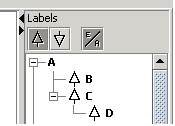
\includegraphics{fig/subtypes-screenshot}
  \end{center}
\end{enumerate}

\paragraph{Type graphs.}

A type graph is itself just an ordinary graph, with a special subtype
edge. Subtype edges are specified (in the editor) as \subP-labelled edges; in
the display view, they are shown as unlabelled edges with an open triangular
arrow point. The subtype edges must define a partial order --- meaning that
there may not be subtype cycles. For instance, the following is a type graph
for the rules and graph in \eqref{subtypes}:

\views{type}
%
If a grammar has a type graph, \GROOVE enforces adherence to it, by flagging as
errors

\begin{itemize}\noitemsep
\item all nodes without types or with more than one type;
\item all node types that do not appear in the type graph;
\item all flags that are not defined in the type graph for the corresponding
  node type, or a supertype thereof;
\item all edges with labels that are not defined in the type graph between the
  corresponding node types, or supertypes thereof;
\item all mergers, and all node type erasers and creators
\end{itemize}
%
For instance, the rules and graph in \eqref{subtypes} an d\eqref{subtypes-alt}
are well-typed with resped to the type graph in \eqref{type}.